During this assignment, the setup in Figure \ref{fig:Ass2_setup} is used. It consists of a pulse generator which sends a square pulse to a DUT (device under test)via a coax cable (with $Z_0 = 50 \Omega$), a sampling unit, which samples the electric field in the coax cable, and an oscilloscope, which measures the sampled electric field strength.\\

\begin{figure}[h]
    \centering
    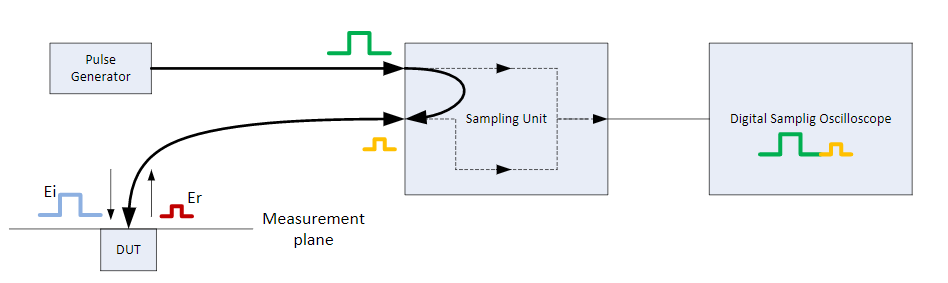
\includegraphics[width=1\textwidth]{Session1_files/Assignment2_setup.PNG}
    \caption{Experimental setup of Assignment 2}
    \label{fig:Ass2_setup}
\end{figure}

\subsection*{Part 1. Time Domain Reflectometry}

In this part, the reflection of an incident square pulse is investigated. As the oscilloscope will measure the total electric field in the coax cable, it will also register the reflection of the pulse, from which the reflection coefficient can be derived.

